\tikzstyle{block} = [rectangle, rounded corners, minimum width=3cm, minimum height=1cm, text centered, draw=black, fill=gray!20]
\tikzstyle{arrow} = [thick,->,>=stealth]
\tikzstyle{double_arrow} = [thick,<->,>=stealth]

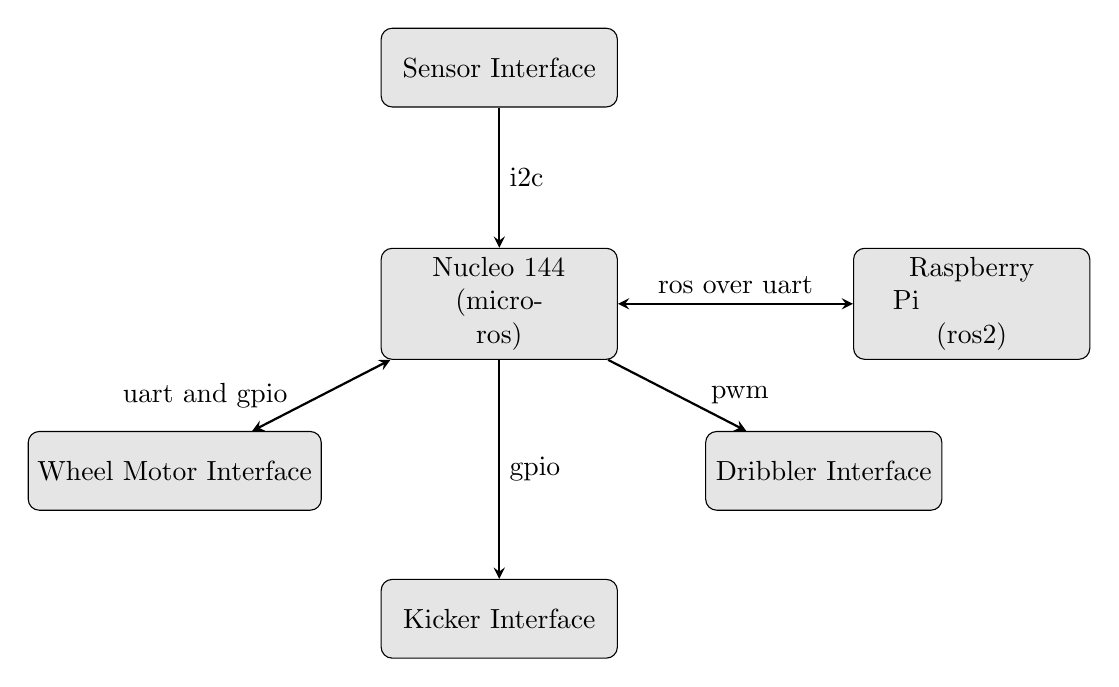
\begin{tikzpicture}[node distance=3cm]

% Nodes
\node (sensors) [block] {Sensor Interface};
\node (nucleo) [block, text width=1.7cm, below of=sensors] {Nucleo 144\newline(\acs{micro-ros})};
\node (raspberry) [block, text width=2cm, right of=nucleo, xshift=3cm] {Raspberry Pi\newline(\acs{ros2})};
\node (wheel) [block, below left of=nucleo, xshift=-2cm] {Wheel Motor Interface};
\node (kicker) [block, below of=nucleo, yshift=-1cm] {Kicker Interface};
\node (dribbler) [block, below right of=nucleo, xshift=2cm] {Dribbler Interface};

% Arrows
\draw [arrow] (sensors) -- (nucleo) node[midway, right] {\acs{i2c}};
\draw [double_arrow] (nucleo) -- (raspberry) node[midway, above] {\acs{ros} over \acs{uart}};
\draw [double_arrow] (nucleo) -- (wheel) node [midway, left, xshift=-0.3cm] {\acs{uart} and \acs{gpio}};
\draw [arrow] (nucleo) -- (kicker) node[midway, right] {\acs{gpio}};
\draw [arrow] (nucleo) -- (dribbler) node[midway, right, xshift=0.3cm] {\acs{pwm}};

\end{tikzpicture}